\documentclass[conference]{IEEEtrans}
\IEEEoverridecommandlockouts
% The preceding line is only needed to identify funding in the first footnote. If that is unneeded, please comment it out.
\usepackage{cite}
\usepackage{amsmath,amssymb,amsfonts}
% \usepackage{algorithmic}
\usepackage{graphicx}
\usepackage{textcomp}
\usepackage{xcolor}
\usepackage{verbatim}
\usepackage{amsmath,amsfonts,mathtools,bm}
\usepackage{geometry}
\usepackage{subfig}
\usepackage{amsthm}
\usepackage{amssymb}
\usepackage{cleveref}
\usepackage{algorithm}
\usepackage{appendix}
% \usepackage{algorithmic}
\usepackage{newclude}
\usepackage{algpseudocode}
\usepackage{tikz} 
\usepackage{appendix}

% \modulolinenumbers[5]


% \def\BibTeX{{\rm B\kern-.05em{\sc i\kern-.025em b}\kern-.08em
%     T\kern-.1667em\lower.7ex\hbox{E}\kern-.125emX}}
\begin{document}

\title{Next Generation Intelligent Spaces\\
% {\footnotesize \textsuperscript{*}Author names are arranged in alphabetical order}
% \thanks{Identify applicable funding agency here. If none, delete this.}
}

% \author{\IEEEauthorblockN{Angan Mitra}
% \IEEEauthorblockA{\textit{Qarnot Computing} \\
% Paris, France \\
% angan.mitra@qarnot-computing.com}
% \and
% \IEEEauthorblockN{ Denis Trystram}
% \IEEEauthorblockA{\textit{Laboratory of Informatics} \\
% Grenoble, France \\
% firstname.lastname@imag.fr}
% }

\maketitle


\begin{abstract}
A building equipped with sensors is a use case of heterogeneous data sources distributed naturally across spaces or zones. Lack of spatiotemporal awareness can lead to excessive sensors or non-optimal distribution across a building. We extend the problem of optimal sensor placement to find the minimal sensor group that can robustly approximate the rest of the sensors values. The solution uses a distributed learning step to parallelize the predictive capability of candidate groups generated by evolutionary computing techniques. Additionally, the system models the cost and energy consumption of the sensor group when performing a multi-objective optimization. We experiment on 24 zones from a seven-storied building in Thailand to establish a trade-off between virtualization accuracy, energy footprint, and installation cost. The work exploits the concept of "less is more" to bring down the capital and recurring expense for a smart building solution.


%  Although there is significant research on Smart Buildings since early 2000's, the rate of embracing the technology is remarkably low. 
%  The main impedance comes from avoiding high-cost industrial grade sensor network installations at households or commercial sites. 
%  A study by behavioural scientists reveal that the break-even period of investing in smart building hardware stands at roughly 5-15 years which often exceed the warranty period of individual components. 
%  Furthermore, there is a dearth of an open source building management system that can generate useful knowledge or insights even from ad-hoc installations on buildings. 

%  In this work, we show a novel mechanism to bring down the cost of operational \textit{smartness} in a building with a sensor agnostic setting. 
%  The methodology yields an energy efficient power allocation policy for illumination and indoor thermal comfort while minimizing the number of sensors used. 
%  Experiments on a real-life data set shows promise on the applicability of such architectures in practical use-cases. 
 
\end{abstract}

\begin{IEEEkeywords}
smart buildings, ambient intelligence, sensor optimization, business intelligence
\end{IEEEkeywords}


\include*{chapters/introduction}
\include*{chapters/relatedwork}
\include*{chapters/formulation}
\include*{chapters/experiments}
\include*{chapters/conclusion}

\section*{Acknowledgment }
This work has been partially supported by the Multi-disciplinary Institute on Artificial Intelligence MIAI at Grenoble Alpes (ANR-19-P3IA-0003) and GRECO project (Resource manager for cloud of things) funded under the reference ANR-16- CE25-0016. Angan Mitra is supported by the convention CIFRE at ANRT 2018/0874. The source code of the work is available at $https://github.com/AnganMitra/ngis/$.


\bibliographystyle{IEEEtran}
\bibliography{ref.bib}

\begin{figure}%
    \centering
    \subfloat[Temperature  ]{{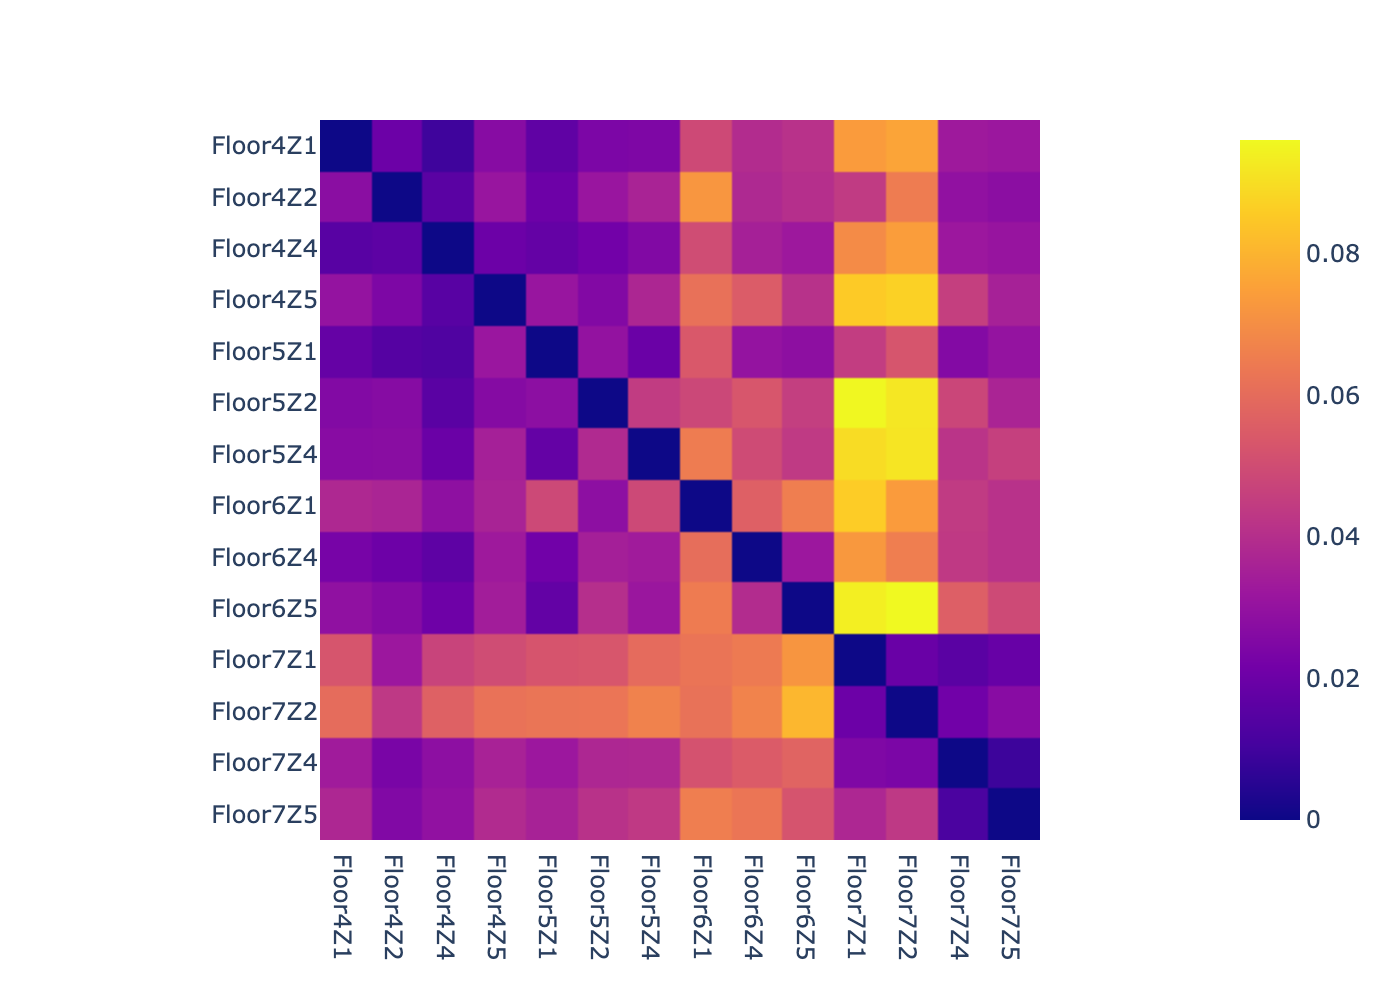
\includegraphics[width=0.47\textwidth]{img/4567fdomain/temperature.png} }}%
    \qquad
    \subfloat[\centering Luminosity levels ]{{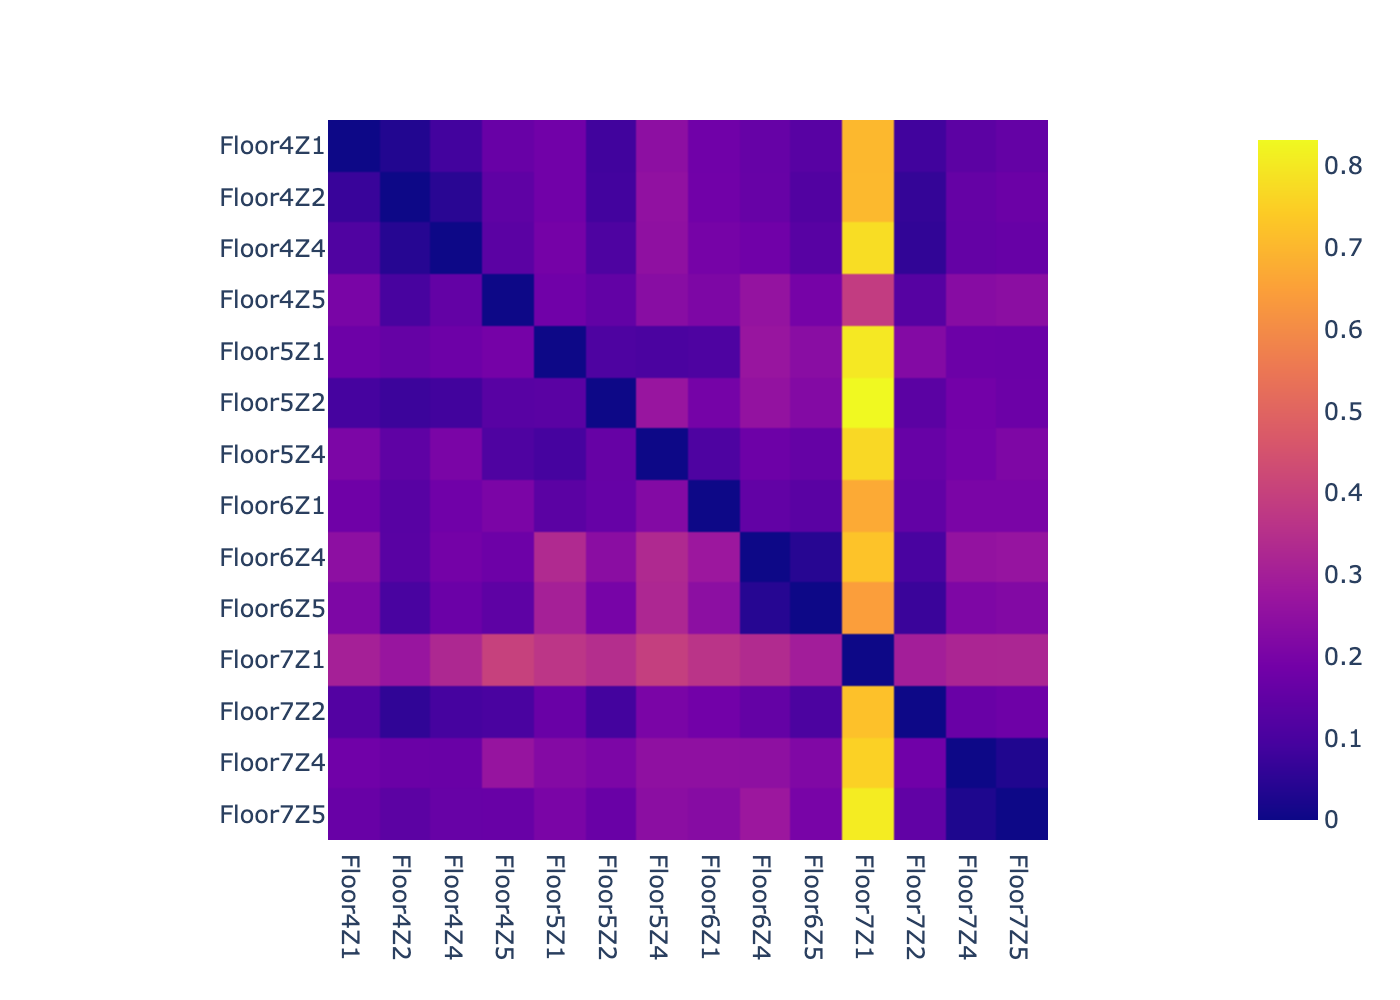
\includegraphics[width=0.47\textwidth]{img/4567fdomain/lux.png} }}%
    \qquad
    \subfloat[\centering Humidity ]{{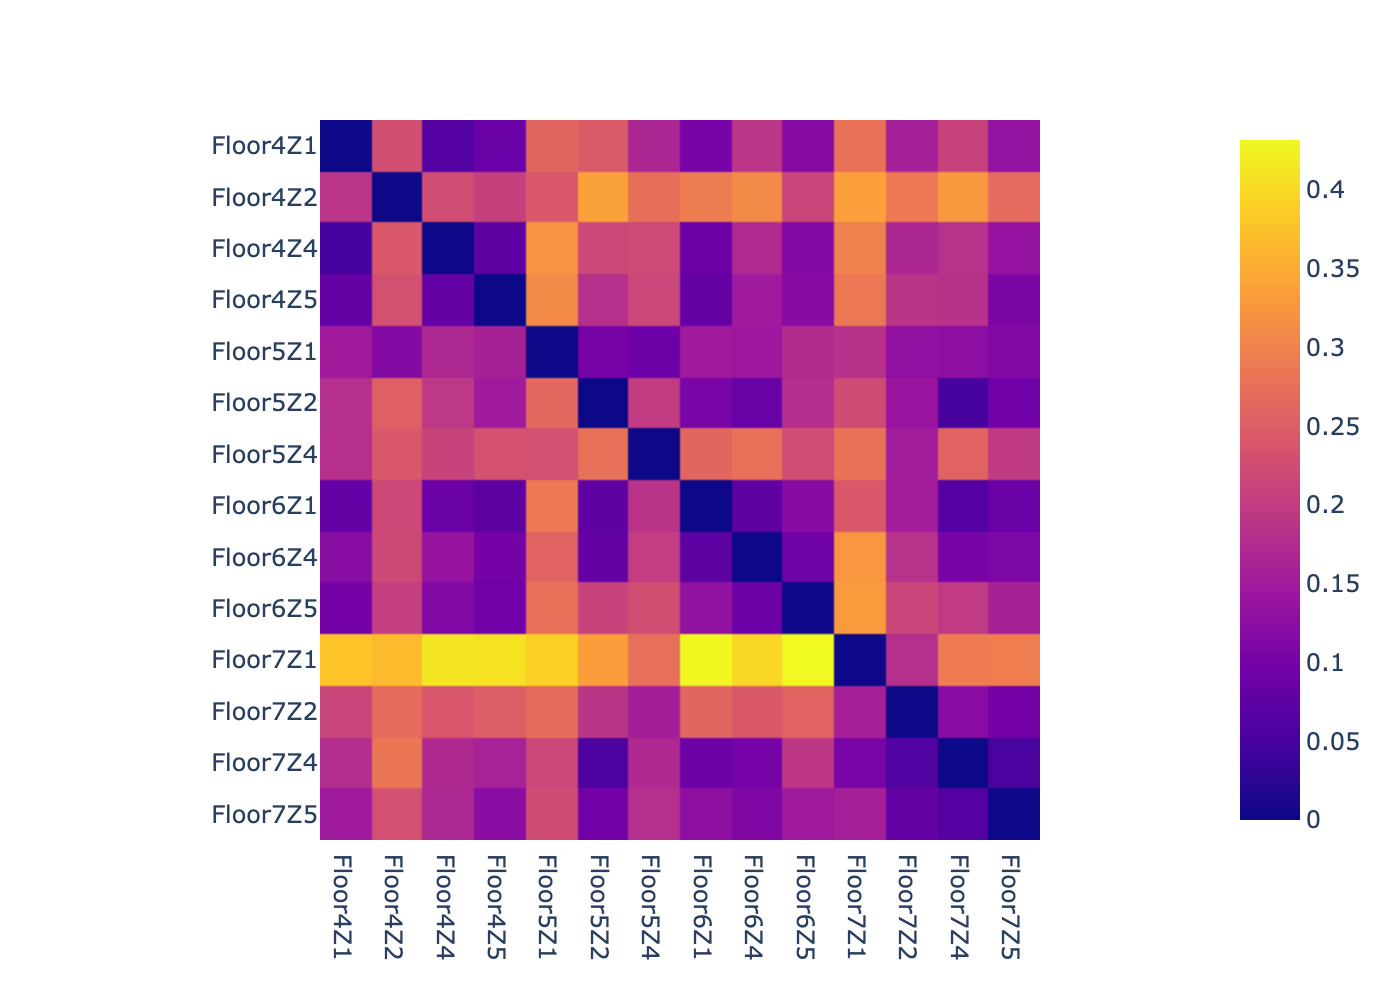
\includegraphics[width=0.47\textwidth]{img/4567fdomain/humidity.png} }}%
    \caption{Virtualization prediction on processing similar ambience channels as one group }%
    \label{fig:domainVirtualizeAmbience}%
\end{figure}

\begin{figure}%
    \centering
    \subfloat[AC Power ]{{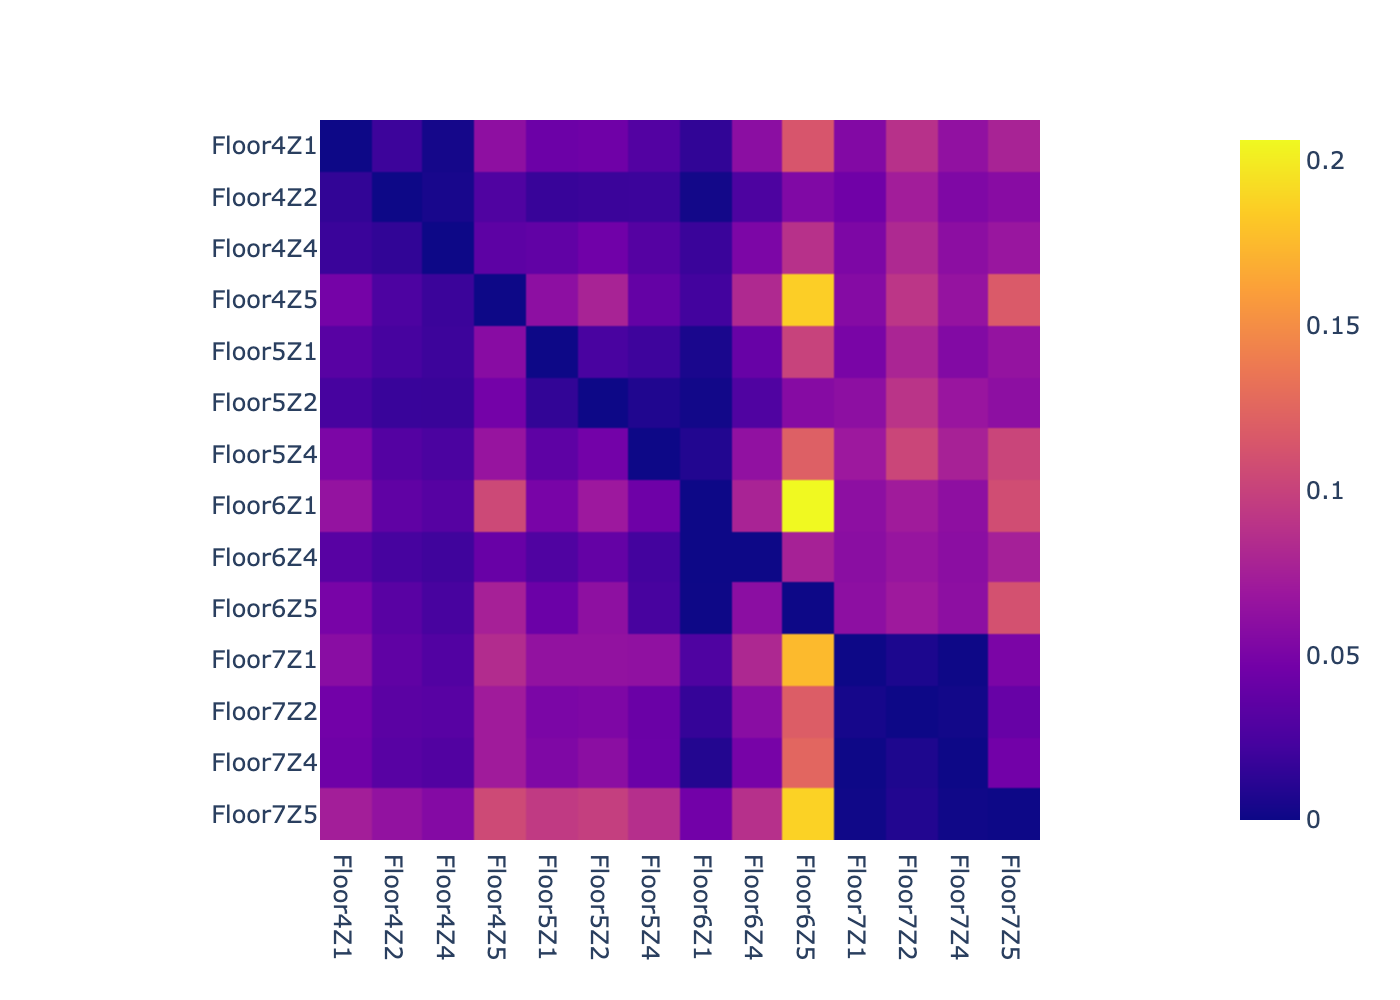
\includegraphics[width=0.47\textwidth]{img/4567fdomain/ACPower.png} }}%
    \qquad
    \subfloat[\centering Light Power] {{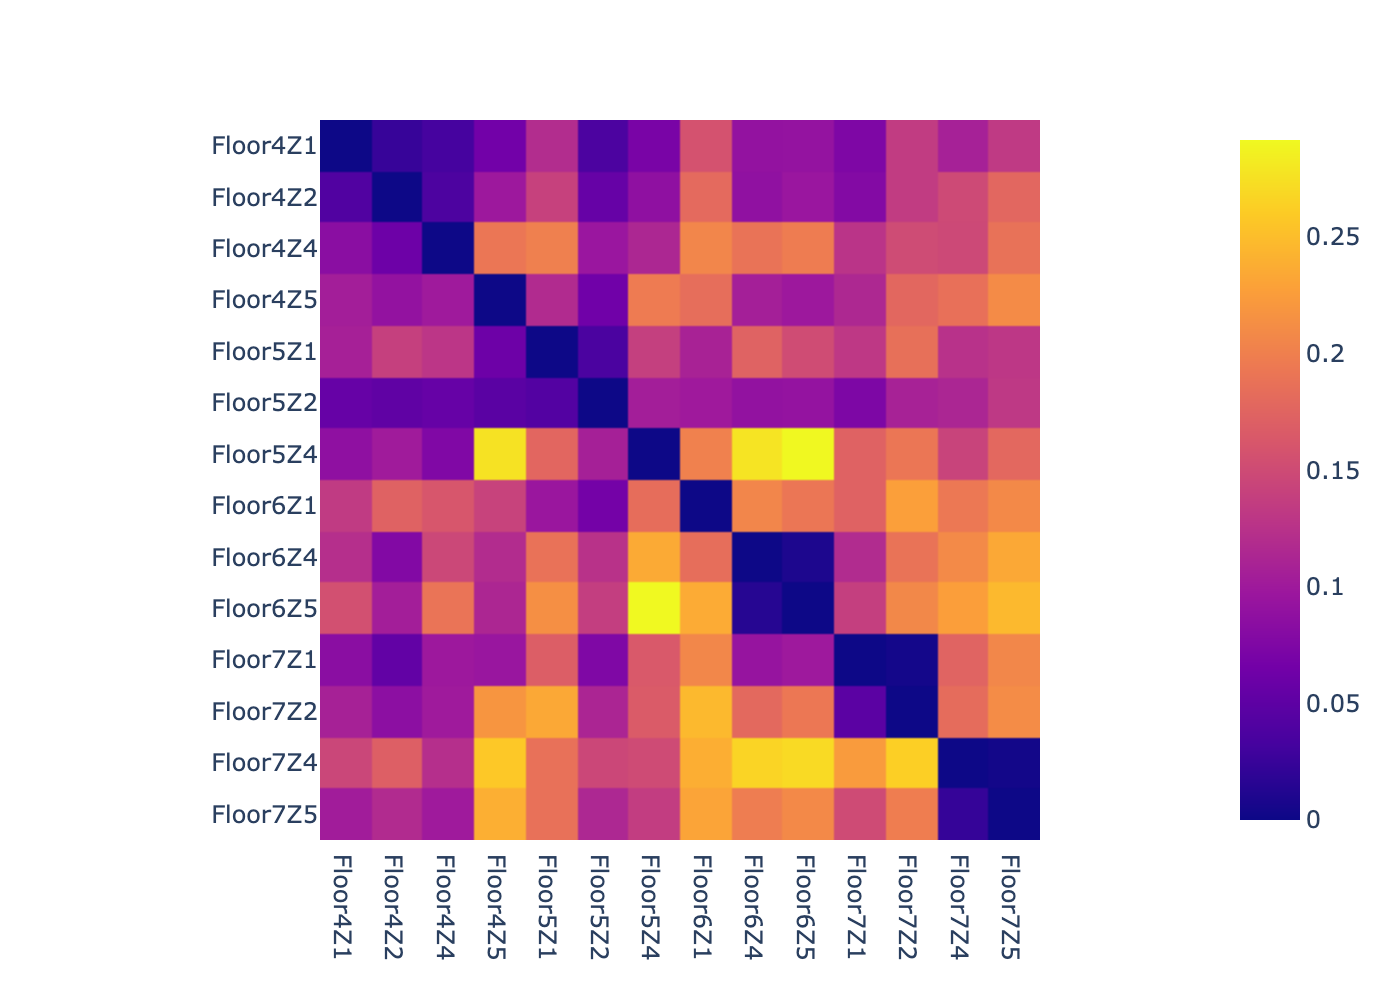
\includegraphics [width=0.47\textwidth] {img/4567fdomain/lightPower.png} }}%
    \qquad
    \subfloat[\centering Appliance Power Consumption ]{{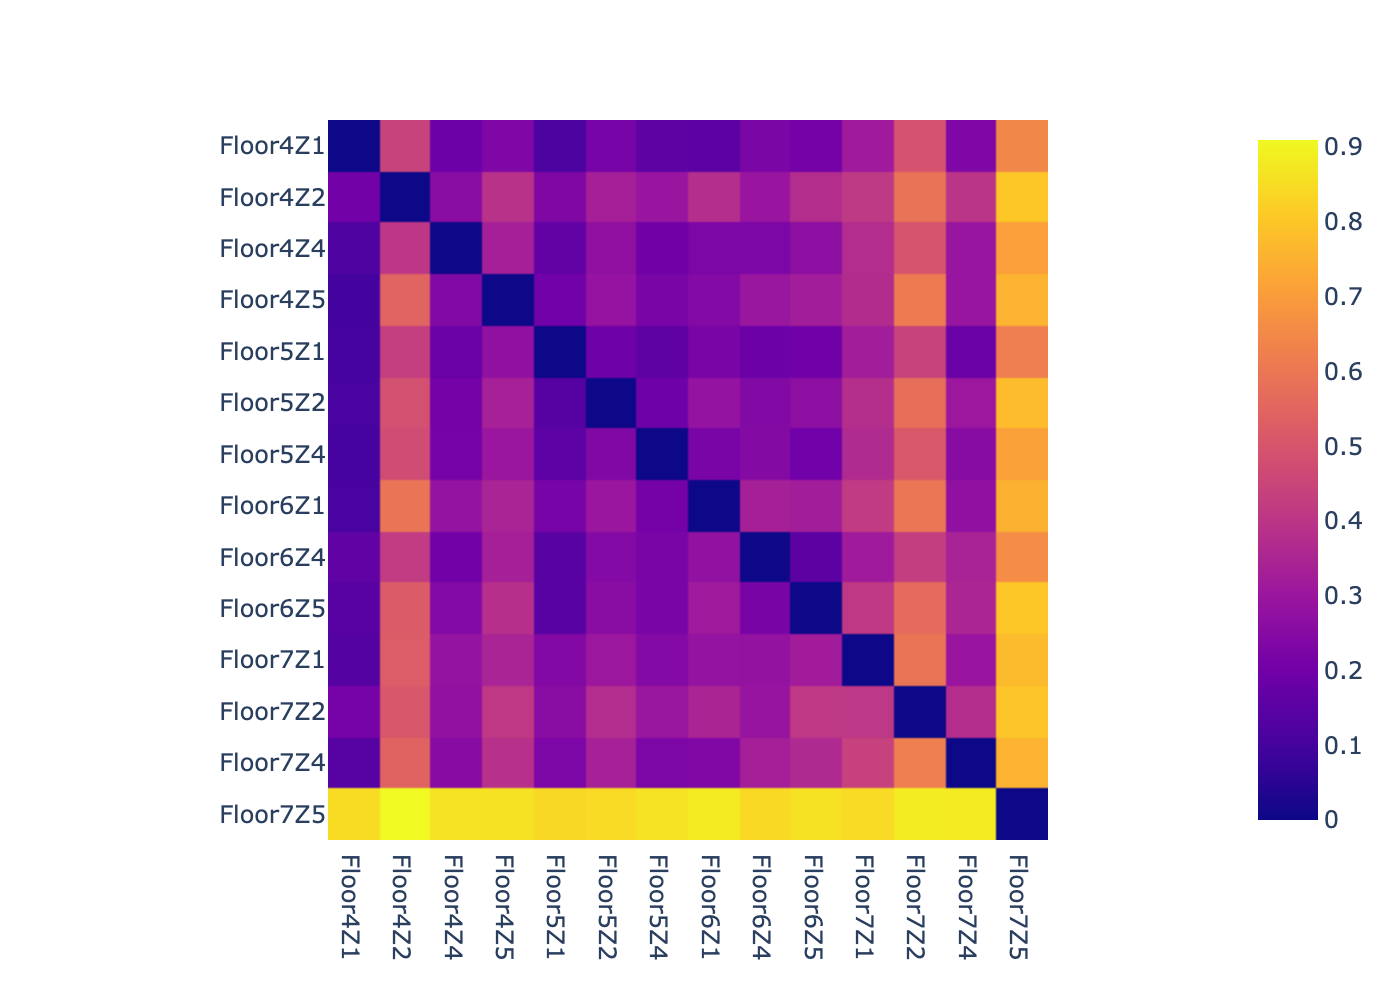
\includegraphics[width=0.47\textwidth]{img/4567fdomain/appPower.png} }}%
    \caption{Virtualization prediction on treating identical type of power meters as one group }%
    \label{fig:domainVirtualizePower}%
\end{figure}



\end{document}
